\documentclass{article}[12pt]
\usepackage{color}
\usepackage[normalem]{ulem}
\usepackage{times}
\usepackage{fullpage}
\usepackage{amsmath}
\usepackage{amssymb}
\usepackage{listings}
\usepackage{tikz}
\def \R {\mathbb R}
\def \imp {\Longrightarrow}
\def \eps {\varepsilon}
\def \Inf {{\sf Inf}}
\newenvironment{proof}{{\bf Proof.  }}{\hfill$\Box$}
\newtheorem{theorem}{Theorem}[section]
\newtheorem{definition}{Definition}[section]
\newtheorem{corollary}{Corollary}[section]
\newtheorem{lemma}{Lemma}[section]
\newtheorem{claim}{Claim}[section]
\setlength {\parskip}{2pt}
\setlength{\parindent}{0pt}

\newcommand{\headings}[4]{\noindent {\bf Midterm CME241} \hfill {{\bf Author:} Nicolas Sanchez} \\
{} \hfill {{\bf SUNETID:} sanchezn} \\

\rule[0.1in]{\textwidth}{0.025in}
}

\newcommand{\klnote}[1]{{\color{red} #1}}
\newcommand{\klsout}[1]{{\color{red} \sout{#1}}}

\begin{document}

\headings{\#1}{Tuesday, October 8, 10:30am}\section{} 



\section{Value Iteration Optimization}
\subsection{Problem Formulation}
We first notice that our entire problem formulation, notably transition probabilities can only be determined once we have the grid make up or specifically a mapping: $$T:\mathbb{N} \times \mathbb{N} \to \{\text{"SPACE","BLOCK","GOAL"}\}$$ Or in words a dictionary which maps from positions on the grid to one of three strings "SPACE", "BLOCK" or "GOAL". Suppose the grid given is of size $n\times m$. Luckily we can make our state space simple regardless of $T$.

\begin{align*}
\mathcal{S} = \{ (i,j) | i,j \in \mathbb{N}, 0\leq i \leq n-1, 0\leq j \leq m-1\}
\end{align*}

Again, the set of terminal states is only known based on the value of $T$. For our design we designate all states that are not "SPACE" as terminal spaces. Although by virtue of the dynamics "BLOCK" states are never reached and thus will never end the process, "BLOCK" states also are never reached and hence do not have well defined transition probabilities. For cleaner computation and to avoid singular behaviors of the transition function we thus have:

\begin{align*}
\mathcal{T} = \{ (i,j) | i,j \in \mathbb{N}, 0\leq i \leq n-1, 0\leq j \leq m-1,T(i,j)\in\{\text{"BLOCK","GOAL"}\}\}\\
\mathcal{N} = \{ (i,j) | i,j \in \mathbb{N}, 0\leq i \leq n-1, 0\leq j \leq m-1,T(i,j) = \text{"SPACE"}\}\}\\
\end{align*}

The possible actions are moving in any of the four directions. We will denote them as "UP", "DOWN", "RIGHT", "LEFT". More compactly for all states we have the constant action set:
$$\mathcal{A} = \{\text{"UP", "DOWN", "RIGHT", "LEFT"\}}$$

For any state $ s\in \mathcal{N}$  and $ s'\in \mathcal{S}$ with $s = (i_s, j_s)$, $s' = (i_{s'}, j_{s'})$, we define the probability distribution in the following cases:

\begin{align*}
\mathcal{P}(s, \text{"DOWN"}, s') &= \begin{cases} \mathbb{I}_{s=s'} \text{  if $i_s = n-1$ or $T(i_s +1, j_s) =$"BLOCK"}\\\mathbb{I}_{i_{s'}=i_s+1, j_{s'}=j_s} \text{ otherwise} \end{cases}\\
\mathcal{P}(s, \text{"UP"}, s') &= \begin{cases} \mathbb{I}_{s=s'} \text{  if $i_s = 0$ or $T(i_s -1, j_s) =$"BLOCK"}\\\mathbb{I}_{i_{s'}=i_s-1, j_{s'}=j_s} \text{ otherwise} \end{cases}\\
\mathcal{P}(s, \text{"RIGHT"}, s')& = \begin{cases} \mathbb{I}_{s=s'} \text{  if $j_s = m-1$ or $T(i_s, j_s+1) =$"BLOCK"}\\\mathbb{I}_{i_{s'}=i_s, j_{s'}=j_s+1} \text{ otherwise} \end{cases}\\
\mathcal{P}(s, \text{"LEFT"}, s') &= \begin{cases} \mathbb{I}_{s=s'} \text{  if $j_s = 0$ or $T(i_s, j_s-1) =$"BLOCK"}\\\mathbb{I}_{i_{s'}=i_s, j_{s'}=j_s-1} \text{ otherwise} \end{cases}
\end{align*}
Note that we are essentially making it so that "illegal moves" that either take the player out of the grid or to a blocked spot simply takes them back to their current state.\\

Finally we propose two reward and discount formulations, $\mathcal{R}_1,\gamma_1$ and  $\mathcal{R}_2, \gamma_2$. For any states $s,s'\in \mathcal{S}$ and action $a\in \mathcal{A}$:
\begin{align*}
\mathcal{R}_1(s, a, s') = -1,\,& \gamma_1 = 1\\
\mathcal{R}_2(s, a, s') = \begin{cases}1 \text{ if $T(i_{s'},j_{s'}) =$"GOAL"}\\ 0 \text{ otherwise}\end{cases},&\, \gamma_2 = 0.5\\
\end{align*}

Both of these formulations should yield the fastest path from start to goal. For formulation 1, every extra step directly reduces the reward by 1 so the optimal solution will take the least steps possible. For formulation 2, every extra step before reaching the end goal means the final reward is halved in value because of the discount factor, hence the optimal solution will take the least steps possible and obtain the least discounted reward.

\subsection{Code}
\begin{lstlisting}
from dataclasses import dataclass
from typing import Callable, Tuple, Iterator, Sequence, List, Mapping, Dict
from rl.markov_decision_process import FiniteMarkovDecisionProcess
from rl.markov_decision_process import FinitePolicy, StateActionMapping
from rl.markov_process import FiniteMarkovProcess, FiniteMarkovRewardProcess
from rl.distribution import Constant, Categorical
from rl.dynamic_programming import value_iteration_result, value_iteration, almost_equal_vfs
from rl.iterate import converge, iterate
from pprint import pprint
import matplotlib.pyplot as plt
import matplotlib
import numpy as np

########## CONSTANTS ##################
SPACE = 'SPACE'
BLOCK = 'BLOCK'
GOAL = 'GOAL'


########## MDP CLASS DEFINITIONS #######################
@dataclass(frozen=True)
class MazeState:
    row: int
    col: int


MazeMoveMapping = StateActionMapping[MazeState, str]

class MazeMovementMDP(FiniteMarkovDecisionProcess[MazeState, str]):

    def __init__(
        self,
        type_dict: Mapping[Tuple[int,int],str],
        rew_fn: Mapping[Tuple[int,int],float],
    ):
        self.type_dict: Mapping[Tuple[int,int],str] = type_dict
        self.grid_size: Tuple[int,int] = (max(type_dict.keys())[0]+1,max(type_dict.keys())[1]+1)
        self.rew_fn: Mapping[Tuple[int,int],float]= rew_fn
        super().__init__(self.get_action_transition_reward_map())

    def get_action_transition_reward_map(self) -> MazeMoveMapping:
        d: Dict[MazeState, Dict[str, Constant[Tuple[MazeState,float]]]] = {}

        # loop through all possible states
        for i_s in range(self.grid_size[0]):
            for j_s in range(self.grid_size[1]):
                if self.type_dict[(i_s,j_s)] != SPACE: continue# do not include terminal states

                s_curr: MazeState = MazeState(i_s, j_s)
                d_s : Dict[str, Constant[Tuple[MazeState,float]]] = {}
                
                ## DOWN ##
                if i_s == self.grid_size[0]-1 or self.type_dict[i_s+1, j_s] == BLOCK:
                    d_s["DOWN"] = Constant((s_curr,self.rew_fn[(i_s,j_s)]))
                else:
                    d_s["DOWN"] = Constant((MazeState(i_s+1, j_s),self.rew_fn[(i_s+1,j_s)]))

                ## UP ##
                if i_s == 0 or self.type_dict[i_s-1, j_s] == BLOCK:
                    d_s["UP"] = Constant((s_curr,self.rew_fn[(i_s,j_s)]))
                else:
                    d_s["UP"] = Constant((MazeState(i_s-1, j_s),self.rew_fn[(i_s-1,j_s)]))

                ## RIGHT ##
                if j_s == self.grid_size[1]-1 or self.type_dict[i_s, j_s+1] == BLOCK:
                    d_s["RIGHT"] = Constant((s_curr,self.rew_fn[(i_s,j_s)]))
                else:
                    d_s["RIGHT"] = Constant((MazeState(i_s, j_s+1),self.rew_fn[(i_s,j_s+1)]))

                ## LEFT ##
                if j_s == 0 or self.type_dict[i_s, j_s-1] == BLOCK:
                    d_s["LEFT"] = Constant((s_curr,self.rew_fn[(i_s,j_s)]))
                else:
                    d_s["LEFT"] = Constant((MazeState(i_s, j_s-1),self.rew_fn[(i_s,j_s-1)]))
                d[s_curr] = d_s
        return d


########## PLOTTING TOOLS #######################
plotting_correspondance = {"NaN":0, "UP": 1, "DOWN": 2,"RIGHT": 3,"LEFT": 4}
plotting_correspondance_rev = ["N/A", "UP", "DOWN","RIGHT","LEFT"]
def discrete_matshow(data, i):
    #get discrete colormap
    cmap = plt.get_cmap('RdBu', np.max(data)-np.min(data)+1)
    # set limits .5 outside true range
    mat = plt.matshow(data,cmap=cmap,vmin = np.min(data)-.5, vmax = np.max(data)+.5)

    #tell the colorbar to tick at integers
    func = lambda x,pos: plotting_correspondance_rev[int(x)]
    cax = plt.colorbar(mat, ticks=np.arange(np.min(data),np.max(data)+1), format = matplotlib.ticker.FuncFormatter(func))
    ax = plt.gca();

    # Major ticks
    ax.set_xticks(np.arange(0, data.shape[0], 1))
    ax.set_yticks(np.arange(0, data.shape[1], 1))

    # Minor ticks
    ax.set_xticks(np.arange(-.5, data.shape[0], 1), minor=True)
    ax.set_yticks(np.arange(-.5, data.shape[1], 1), minor=True)

    # Gridlines based on minor ticks
    ax.grid(which='minor', color='w', linestyle='-', linewidth=2)
    plt.show()


################# IMPLEMENTATION TO GIVEN MAZE DICTIONARY ########################
if __name__ == '__main__':

    maze_grid = {(0, 0): SPACE, (0, 1): BLOCK, (0, 2): SPACE, (0, 3): SPACE, (0, 4): SPACE, 
             (0, 5): SPACE, (0, 6): SPACE, (0, 7): SPACE, (1, 0): SPACE, (1, 1): BLOCK,
             (1, 2): BLOCK, (1, 3): SPACE, (1, 4): BLOCK, (1, 5): BLOCK, (1, 6): BLOCK, 
             (1, 7): BLOCK, (2, 0): SPACE, (2, 1): BLOCK, (2, 2): SPACE, (2, 3): SPACE, 
             (2, 4): SPACE, (2, 5): SPACE, (2, 6): BLOCK, (2, 7): SPACE, (3, 0): SPACE, 
             (3, 1): SPACE, (3, 2): SPACE, (3, 3): BLOCK, (3, 4): BLOCK, (3, 5): SPACE, 
             (3, 6): BLOCK, (3, 7): SPACE, (4, 0): SPACE, (4, 1): BLOCK, (4, 2): SPACE, 
             (4, 3): BLOCK, (4, 4): SPACE, (4, 5): SPACE, (4, 6): SPACE, (4, 7): SPACE, 
             (5, 0): BLOCK, (5, 1): BLOCK, (5, 2): SPACE, (5, 3): BLOCK, (5, 4): SPACE, 
             (5, 5): BLOCK, (5, 6): SPACE, (5, 7): BLOCK, (6, 0): SPACE, (6, 1): BLOCK, 
             (6, 2): BLOCK, (6, 3): BLOCK, (6, 4): SPACE, (6, 5): BLOCK, (6, 6): SPACE, 
             (6, 7): SPACE, (7, 0): SPACE, (7, 1): SPACE, (7, 2): SPACE, (7, 3): SPACE, 
             (7, 4): SPACE, (7, 5): BLOCK, (7, 6): BLOCK, (7, 7): GOAL}

    rew1: Mapping[Tuple[int,int],float] = {k:-1 for k in maze_grid.keys()}
    gamma1 = 1.0
    rew2: Mapping[Tuple[int,int],float] = {k: 1 if maze_grid[k] == GOAL else 0 for k in maze_grid.keys()}
    gamma2 = 0.5


    forms_list = [(rew1,gamma1),(rew2, gamma2)]#[(rew1, gamma1)]#
    for i, tup  in enumerate(forms_list):
        rew, gamma = tup
        maze_mdp: FiniteMarkovDecisionProcess[MazeState, str] =\
            MazeMovementMDP(
                type_dict = maze_grid,
                rew_fn = rew
            )
        print("MDP Value Iteration Optimal Policy and Number of Iterations For Formulation "+ str(i+1))
        print("--------------")
        opt_vf_vi, opt_policy_vi = value_iteration_result(maze_mdp, gamma=gamma)
        plotted_opt_pl = np.zeros(maze_mdp.grid_size)
        for s in opt_policy_vi.states():
            plotted_opt_pl[s.row,s.col] = plotting_correspondance[opt_policy_vi.act(s).sample()]
        pprint(plotted_opt_pl)
        discrete_matshow(plotted_opt_pl,i)
        print("NUMBER OF ITERATIONS", len([1 for _ in converge(value_iteration(maze_mdp, gamma=gamma), done = almost_equal_vfs)]))
    \end{lstlisting}

\subsection{Results}
Plotting the two optimal policies confirms they are the same and the number of iterations need in value iteration are both  17 iterations so they are equally fast. See plots below.

\begin{figure}
  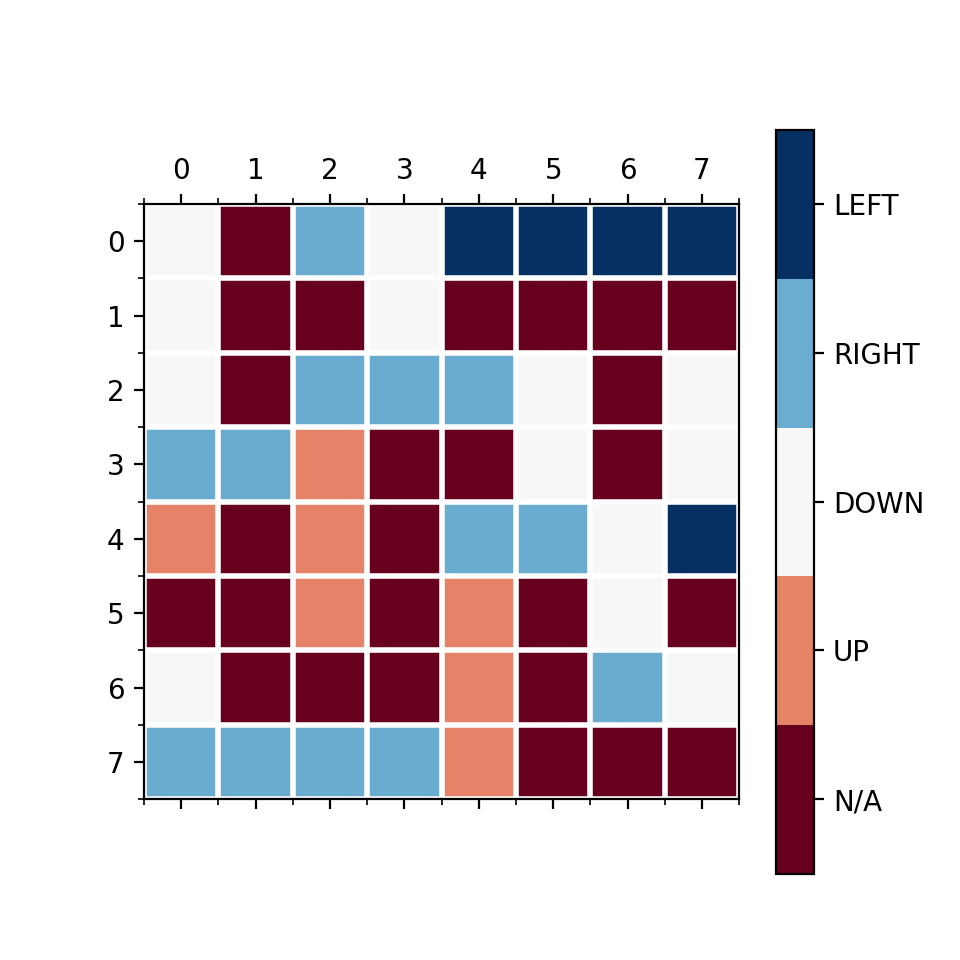
\includegraphics[width=\linewidth]{opt_pol_form1.png}
  \caption{Optimal Policy For Problem Formulation 1}
  \label{fig:optPol1}
\end{figure}
\begin{figure}
  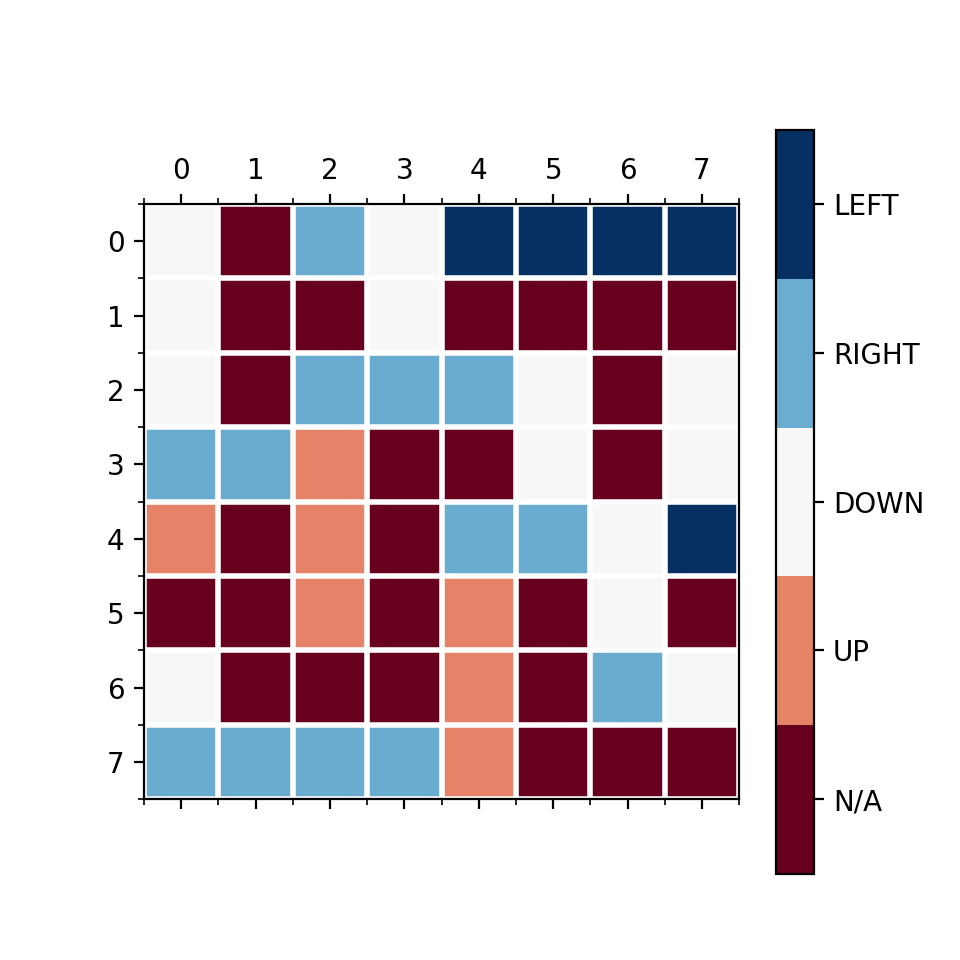
\includegraphics[width=\linewidth]{opt_pol_form2.png}
  \caption{Optimal Policy For Problem Formulation 2}
  \label{fig:optPol2}
\end{figure}

\section{MRP Value Function Approximation}
With the given forms for $(\mathcal{S},\mathcal{P},\mathcal{R}, \gamma)$: 

\begin{align*}
\mathcal{P} &\in \mathbb{R}^{n\times n}\\
\mathcal{R} &\in \mathbb{R}^{n}\\
\gamma &\in \mathbb{R}\\
\end{align*} 

we know from lecture the expression for the value function $\mathcal{V} \in \mathbb{R}^n$:

\begin{align*}
\mathcal{V} & =\mathcal{R}  + \gamma \mathcal{P}\mathcal{V} \\
\mathcal{V}  &=(I - \gamma \mathcal{P})^{-1} \mathcal{R}
\end{align*} 

On the other hand we seek to linearly approximate $\mathcal{V}$ using $\Phi \in \mathbb{R}^{n\times m}$ which formally means we look for the optimal weights $w\in \mathbb{R}^m$ such that:
\begin{align*}
\mathcal{V} \approx \Phi w
\end{align*}

Exact representation under this family of approximations is therefore equivalent to stating there exists a $w \in \mathcal{R}^m$ :
\begin{align*}
\mathcal{V} =\Phi w &= (I - \gamma \mathcal{P})^{-1} \mathcal{R}\\
\end{align*}
which rearranging yields (to avoid matrix inversions):
\begin{align*}
(I - \gamma \mathcal{P})\Phi w &= \mathcal{R}\\
\end{align*}
This in turn is exactly equivalent to requiring that the reward vector is in the linear span of the matrix $(I - \gamma \mathcal{P})\Phi$.
 $$ \mathcal{R} \in \text{span}((I - \gamma \mathcal{P})\Phi) = \{(I - \gamma \mathcal{P})\Phi w | w\in\mathbb{R}^m\}$$
 Or if we want a condition purely on $\Phi$:
  $$(I - \gamma \mathcal{P})^{-1}R \in \text{span}(\Phi)$$
 We can further restate this as the condition that there exists a solution $x\in \mathbb{R}^m$ to the equation:
 $$ (I - \gamma \mathcal{P})\Phi x = \mathcal{R}$$
 
Since these two facts are both necessary and sufficient for the linear approximation to exactly recreate $V$, we know that these are minimal conditions for $\Phi$ given $(\mathcal{S},\mathcal{P},\mathcal{R}, \gamma)$.
 
\section{Career Optimization}
\subsection{Problem Formulation}
We construct the MDP formulation as follows. The state is completely determined by the wage level.
$$ \mathcal{S} = \{w|w\in\mathbb{N}^+, w\leq W\}$$ 
 
The actions are the allocations of time $l,s$ within the constraint on any given day or more precisely:
$$ \mathcal{A} = \{(l,s) | l,s\in\mathbb{N}, l+s \leq H\}$$

The reward will be the employee payout on that given day, or more precisely:
$$R(w, (l,s), w') = w(H-l-s)$$

We now turn to the more involved process of understanding transition probabilities $P(w,(l,s),w')$. We go through the different cases of $w,w'$ pairs. We will denote $D_{\alpha l}(x)$ as $P(X = x)$ for $X\sim Poi(\alpha l)$ or the probability mass function for a poisson random variable with mean $\alpha l$ and $C_{\alpha l}(x)$ as $P(X \leq x)$ for $X\sim Poi(\alpha l)$ or the cumulative distribution function for a poisson random variable with mean $\alpha l$. \\

If $w>w'$ then probability is trivially 0 as wages will never go down in this dynamic.\\
If $w' = w$, then the employee received no upping in wage which implies he simultaneously did not get offered a job away (this happens with probability $1-\frac{\beta s}{H}$) and did not get paid more because of his learning (this happens with probability $D_{\alpha l}(0)$).\\
If $w' =w+1$ and $w'<W$, then the employee either received a up in pay do to learning of 1 unit (with probability $D_{\alpha l}(1)$) or simultaneously received a different job offer (with probability $\frac{\beta s}{H}$) and no up in pay due to learning (with probability $D_{\alpha l}(0)$).\\
If $w'=w+1$ and $w'=W$, then the employee must have received an up in pay do to learning of at least $1$ unit (with probability $1-C_{\alpha l}(w'-w-1)$) or simultaneously received a different job offer (with probability $\frac{\beta s}{H}$) and no up in pay due to learning (with probability $D_{\alpha l}(0)$).\\
If $w'>w+1$ and $w'<W$, then the employee must have received an up in pay do to learning of $w'-w$ units (with probability $D_{\alpha l}(w'-w)$).\\
If $w'>w+1$ and $w'=W$, then the employee must have received an up in pay do to learning of at least $w'-w$ units (with probability $1-C_{\alpha l}(w'-w-1) = 1-C_{\alpha l}(w'-w) + D_{\alpha l}(w-w')$).\\

We can summarize our results:
$$ P(w,(l,s), w') = \begin{cases}D_{\alpha l}(w'-w) + \mathbb{I}_{w' = W}(1-C_{\alpha l}(w'-w)) +  \mathbb{I}_{w' = w+1}\frac{\beta s}{H}D_{\alpha l}(0)  &\text{ if $w'>w$}\\ (1-\frac{\beta s}{H})D_{\alpha l}(0)  &\text{ if $w'=w$}\\ 0 &\text{ otherwise} \end{cases}$$

Finally we use the daily discount factor as the given discount factor for the MDP $\gamma$.

\subsection{Code}
\begin{lstlisting}
from dataclasses import dataclass
from typing import Callable, Tuple, Iterator, Sequence, List, Mapping, Dict
from rl.markov_decision_process import FiniteMarkovDecisionProcess
from rl.markov_decision_process import FinitePolicy, StateActionMapping
from rl.markov_process import FiniteMarkovProcess, FiniteMarkovRewardProcess
from rl.distribution import Constant, Categorical
from rl.dynamic_programming import value_iteration_result, value_iteration, almost_equal_vfs
from pprint import pprint
from scipy.stats import poisson

########## MDP CLASS DEFINITIONS #######################
@dataclass(frozen=True)
class CareerState:
    wage: int

CareerLadderMapping = StateActionMapping[CareerState, Tuple[int,int]]

class CareerMDP(FiniteMarkovDecisionProcess[CareerState, Tuple[int,int]]):

    def __init__(
        self,
        daily_hours_H: int,
        max_wage_W: int,
        alpha: float,
        beta: float
    ):
        self.daily_hours_H: int = daily_hours_H
        self.max_wage_W: int = max_wage_W
        self.alpha: float = alpha
        self.beta: float = beta
        super().__init__(self.get_action_transition_reward_map())

    def get_action_transition_reward_map(self) -> CareerLadderMapping:
        d: Dict[CareerState, Dict[Tuple[int,int], Categorical[Tuple[CareerState,float]]]] = {}
        for curr_wage in range(1,self.max_wage_W+1):
            state_curr: CareerState = CareerState(curr_wage)
            d_s : Dict[Tuple[int,int], Categorical[Tuple[CareerState,float]]] = {}
            
            # create all possible actions
            for learn_hours in range(self.daily_hours_H+1):
                lambda_curr = float(learn_hours)*self.alpha
                for search_hours in range(self.daily_hours_H+1 - learn_hours):
                    p_job_offer = self.beta*float(search_hours)/float(self.daily_hours_H)
                    # reward is only dependent on action and current state so can compute that first
                    reward_daily = float((self.daily_hours_H - learn_hours - search_hours)*curr_wage)
                    
                    # next we need to check probability of all wage increases
                    next_wage_probs_dict : Dict[Tuple[CareerState, float], float] = {}
                    
                    # first case of no incremental wage
                    next_wage_probs_dict[(CareerState(curr_wage), reward_daily)] =\
                     (1.-p_job_offer)*poisson.pmf(0,lambda_curr)

                    # then all incremental wages cases as outlined in pdf
                    for add_wage in range(1,self.max_wage_W+1-curr_wage):
                        prob_trsn = poisson.pmf(add_wage,lambda_curr)
                        if add_wage ==1:
                            prob_trsn +=poisson.pmf(0,lambda_curr)*p_job_offer
                        if curr_wage+add_wage == self.max_wage_W:
                            prob_trsn += 1.-poisson.cdf(add_wage,lambda_curr)
                        next_wage_probs_dict[(CareerState(curr_wage+add_wage), reward_daily)] =prob_trsn

                    # construct transition for given state+action
                    d_s[(learn_hours,search_hours)] = Categorical(next_wage_probs_dict)
            d[state_curr] = d_s
        return d


################# IMPLEMENTATION ########################
if __name__ == '__main__':
    alpha = 0.08
    beta = 0.82
    gamma = 0.95
    H = 10
    W = 30

    # create MDP
    career_mdp: FiniteMarkovDecisionProcess[CareerState, Tuple[int,int]] =\
        CareerMDP(
        daily_hours_H= H,
        max_wage_W=W,
        alpha= alpha,
        beta=beta
        )

    # perform optimization
    opt_vf_vi, opt_policy_vi = value_iteration_result(career_mdp, gamma=gamma)

    #print out result
    print(opt_policy_vi)
   \end{lstlisting}

\subsection{Results}
Printing out the resulting optimal policy yields dedicating all of your time to learning until obtaining a job with wage greater than $13$ and then dedicating all of your time to searching for a job until getting a job with wage greater than $15$, and finally for higher wages just work all the possible hours.\\

Intuitively this makes sense as follows - if there is potential for significantly greater earning, because of the discount factor, you want to be getting that significant amount more faster and if current wage is low you are not missing out on much by not working. Learning is the vehicle with most chances of achieving a quick rise in wages (with these choices of alpha and beta) when there are chances of much higher wages aka when your current wage is very small (in this case less than 13), so might as well maximise the chances of getting that increase rather than spend time in suboptimal state. Once there is no significant potential for wage growth (wage greater than 15) it is better to just spend all of the time working and obtaining high wages now vs later (given discount factor) rather than wasting time not working, potentially missing out on wages for a while (more valuable wages given discount!). There is a middle ground where you are willing to not work and potentially forego some higher wages (13-15) but want more assurance that you are only doing this for a small period of time, that is to say with more likelihood you at least get a slightly better wage. Hence you maximise by only searching for a job which does just that. The print out is below:

\begin{lstlisting}
For State CareerState(wage=1):
  Do Action (10, 0) with Probability 1.000
For State CareerState(wage=2):
  Do Action (10, 0) with Probability 1.000
For State CareerState(wage=3):
  Do Action (10, 0) with Probability 1.000
For State CareerState(wage=4):
  Do Action (10, 0) with Probability 1.000
For State CareerState(wage=5):
  Do Action (10, 0) with Probability 1.000
For State CareerState(wage=6):
  Do Action (10, 0) with Probability 1.000
For State CareerState(wage=7):
  Do Action (10, 0) with Probability 1.000
For State CareerState(wage=8):
  Do Action (10, 0) with Probability 1.000
For State CareerState(wage=9):
  Do Action (10, 0) with Probability 1.000
For State CareerState(wage=10):
  Do Action (10, 0) with Probability 1.000
For State CareerState(wage=11):
  Do Action (10, 0) with Probability 1.000
For State CareerState(wage=12):
  Do Action (10, 0) with Probability 1.000
For State CareerState(wage=13):
  Do Action (10, 0) with Probability 1.000
For State CareerState(wage=14):
  Do Action (0, 10) with Probability 1.000
For State CareerState(wage=15):
  Do Action (0, 10) with Probability 1.000
For State CareerState(wage=16):
  Do Action (0, 0) with Probability 1.000
For State CareerState(wage=17):
  Do Action (0, 0) with Probability 1.000
For State CareerState(wage=18):
  Do Action (0, 0) with Probability 1.000
For State CareerState(wage=19):
  Do Action (0, 0) with Probability 1.000
For State CareerState(wage=20):
  Do Action (0, 0) with Probability 1.000
For State CareerState(wage=21):
  Do Action (0, 0) with Probability 1.000
For State CareerState(wage=22):
  Do Action (0, 0) with Probability 1.000
For State CareerState(wage=23):
  Do Action (0, 0) with Probability 1.000
For State CareerState(wage=24):
  Do Action (0, 0) with Probability 1.000
For State CareerState(wage=25):
  Do Action (0, 0) with Probability 1.000
For State CareerState(wage=26):
  Do Action (0, 0) with Probability 1.000
For State CareerState(wage=27):
  Do Action (0, 0) with Probability 1.000
For State CareerState(wage=28):
  Do Action (0, 0) with Probability 1.000
For State CareerState(wage=29):
  Do Action (0, 0) with Probability 1.000
For State CareerState(wage=30):
  Do Action (0, 0) with Probability 1.000
\end{lstlisting}

\end{document}
